\clearpage
\section{Analysis} \label{sec:analysis}
The analysis section will be split into different segments: Container technology, Kubernetes, the IoT/edge stack, and, finally, the requirements for the implementation. Essentially, the analysis will be the foundation of the implementation giving reason to the major design choices described in the requirements. The critical areas for the edge are: memory and disk space constrains, security, speed, protocols, loadbalancing and internet access.

In this thesis I will deploy containers to the edge using Kubernetes to determine what is still missing and what features already enable Kubernetes to make this possible. Standardization of the edge is going to be key.

\subsection{Use Cases}
Kubernetes can be installed on most devices running Linux including many single-board computers like the Raspberry Pi. Using Kubernetes comes with the benefit of full orchestration from the cloud. That means, once a desired state is provided to the Kubernetes master it will work towards achieving this desired state. If the system leaves the desired state, Kubernetes will actively try to restore it. 

The main downside of this is the processing overhead. Containers, the main deployment method of applications in Kubernetes have been shown to have little overhead over native applications, see \cref{sec:containers}. Thus, if an IoT gateway has sufficient resources to run Kubernetes and if the system does not have real time requirements, then Kubernetes can be an excellent choice. Following are two use cases for Kubernetes.


\subsubsection{Use Case 1: Smart Stores}
Smart stores have many cameras and sensors monitoring the consumers and items. This data needs to be constantly analyzed and converted into meta data. This meta data needs to be constantly available to all nodes inside the cluster.

The IoT gateways used in the store are heterogeneous, some are based on ARM and others on x86\_64. They also differ in processing power, network connection, the number of applications they run and the IoT devices they are connected to. Some of the IoT devices run on battery and have very limited processing power. There are system relevant applications which need to be always running. Others are for telemterics and non business related purposes and are not system critical.

The store also maintains some legacy apps which should be integrated into the cluster. For these application it is important that the traffic can be controlled without actually changing the application code.

As the store changes its offerings and layout the gateways are used to deploy a wide variety of  applications. Developers adding features to an application also deploy the new application, but are not able to change other resources. To ease the administration the store sets the configuration in the cloud and lets the system do the update. 

All applications and nodes have to be constantly working and one crash or malicious attack should not jeoperdize the entire system.

\subsubsection{Use Case 2: Ticket Terminal}
A cinema chain has a ticket terminals where the user can create an account and set his credit card details and other user data. The terminals are placed in each cinema and upload the user data to the cloud for centralized storage. Thus, a user in cinema A can also automatically check in in cinema B. The terminals also have a card reader for easier check in. Every year the card reader manufacturer produces an update for the devices. These updates are deployed on the terminals via the central configuration point.

Because of GDPR purposes all communication between card reader and the terminal and the cloud and the terminals is encrypted. The applications are also only able to communicate with the cloud.
The cinema company also made sure that the terminal and application are secure and that only trusted applications run on the terminal.

All terminals work independently from each other but run the same application code. Each month the design of the application is changed to represent new movies. The developers build a new image and push it to a registry. They then tell the system to deploy the new version.

\comment{
Since edge devices can also produce terabytes of data, taking the analytics closer to the source of the data on the edge can be more cost-effective by analyzing data near the source and only sending small batches of condensed information back to the centralized systems.
}

\subsection{Requirements Specification}
The requirements are based on insights from existing solutions and the use cases and provide a guideline for the implementation in the next section. I will only create functional requirements as non-functional requirements "indirectly related to the overall success of the system"\cite{aauFunctionalRequirements} and are usually confirmed by intense testing. As this thesis aim is to provide an exploratory example of using Kubernetes at the edge specific constraints are not important. 

The functional requirements are listed and ordered via the MoSCoW method in \cref{tab:functionalRequirements}. The main purpose in this thesis is to have a working prototype showcasing Kubernetes on the edge. The MUST requirements are the once deemed necessary to fulfill this and have a "M" (for MUST) in the "Class" field of the table. The SHOULD requirements are abbreviated by "S" are features which do not make or brake the system, but for an industry wide standard they should be present. This mainly includes security and networking aspects. The COULD requirements are mainly features which add extra business functionality and make the system easier to use. The WOULD requirements are features which are either not directly related to the product or out of scope.
% Please add the following required packages to your document preamble:
% \usepackage[normalem]{ulem}
% \useunder{\uline}{\ul}{}
% \begin{table}[]
\clearpage
\setlength\LTleft{-2.5cm}
\begin{longtable}{l p{3.5cm} p{0.8cm} p{12.5cm} }
\multicolumn{4}{l}{Functional Requirements}       
                                                                                                                                                                                                                              \\
ID                      & Name                                    & Class  & Description                                                                                                                                                                                                                         \\ \hline




101                     & Isolated applications                   & M      & Each application has to function on its own. It has to handle database errors and communication errors in a non fatal way.                                                                                                          \\
102                     & Isolation to host computer              & M      & The application has to be as isolated from the host environment as possible.                                                                                                                                                        \\
103                     & Minimal dependencies                    & M      & The application has to have minimal runtime dependencies. If the application is built on the edge device the compile time dependencies have to be minimal as well.                                                                  \\
104                     & Cross compilation                       & M      & The edge applications has to be able to be cross-compiled.                                                                                                                                                                          \\
105                     & Small images                            & M      & The footprint of the application has to be small as possible                                                                                                                                                                        \\
106                     & Use different users                     & M      & Each application should be run by different users. If one userspace is compromised it does not effect the other applications.                                                                                                       \\
107                     & Use non root user                       & M      & The application should not run with root priviledges except when really needed.                                                                                                                                                     \\
108                     & Isolate the application context         & M      & The application process has to be isolated. Only if the application must access host resources should they be available to the application.                                                                                         \\
109                     & Secured application code                & M      & The application source code has to be secure in case of a databreach on the node. A malicious attacker should not be able to reconstruct the source code even when he gets access to it.                                            \\
110                     & Trusted applications                    & W      & The edge application would be verified before the deployment.                                                                                                                                                                       \\
111                     & Centralized orchestration               & M      & The operator should only need to tell a central configuration tool in the cloud how the system should looks like. The cloud has to then orchestrate the edge automatically.                                                         \\
112                     & Automatic application deployment        & M      & Based on a new configuration the edge device has to be able to automatically get a copy of the new application shut down the old application and deploy the new one.                                                                \\
113                     & Isolate edge from cloud                 & C      & The cloud and the edge could work independently so without a data connection. This is in case the edge is powerful enough to run its own control plane and the setup is big enough to justify the overhead of running multicluster. \\
114                     & Isolated cloud environments             & S      & Developers should only have access to the resources they need.                                                                                                                                                                      \\
115                     & Resource quotas                         & M      & The operators must be able to set resource quotas on applications and groups of applications.                                                                                                                                       \\
116                     & ARM compatible edge                     & M      & The orchestration tool on the edge has to be able to run on (slower) ARM powered devices.                                                                                                                                           \\
117                     & Node fault tolerance                    & M      & The state of each node must be synchronized in the system so that in case of an error the last operable state can be recovered.                                                                                                     \\
118                     & Decentralized edge storage              & W      & When possible each edge device would synchronization important data with other edge devices in a distributed database.                                                                                                              \\
119                     & Traffic prioritization                  & S      & System critical information should be prioritized in case of congestion.                                                                                                                                                            \\
120                     & Whitelist connections                   & S      & Only cluster internal communication should be allowed to access applications on the pods.                                                                                                                                           \\
121                     & Application independent traffic shaping & S      & The traffic for each application should be contralable without changing the application code.                                                                                                                                       \\
122                     & Secure traffic within cluster           & S      & The communication between the nodes inside the cluster should be secure. This includes the edge to cloud communication.                                                                                                             \\
123                     & Internet compatible IoT protocol        & M      & The IoT protocol must to be compatible with the Internet protocol. This enables addressing of IoT devices through the Internet in case of a static IP.                                                                              \\
124                     & Secure traffic with IoT devices         & S      & The communication between the IoT gateway/edge device and the IoT device needs to be secure.                                                                                                                                        \\
125                     & Efficient message compression           & M      & The messages between the edge device and the IoT device must be efficiently compressed to save resource and enhance speed.                                                                                                          \\
126                     & Energy efficient transmission           & M      & The transmission between the edge and the IoT device must be energy efficient.                                                                                                                                                      \\
127                     & Automatic updates                       & S & The edge device should be able to update the IoT device. The update process is intiated in the cloud but the operator does not have to do local configurations. The system updates alone once initiated.                            \\
128                     & OTA updates                             & C      & The IoT device updates could support OTA updates.                                                                                                                                                                                   \\
129                     & Verified updates                        & W  & The IoT device updates would be verified before installing them.                                                                                                                                                                   




\end{longtable}
\label{tab:functionalRequirements}
% \end{table}
\clearpage

\comment{
First list and then clissify (MoSCoW

An example of a functional requirement would be:
A system must send an email whenever a certain condition is met (e.g. an order is placed, a customer signs up, etc).

Docker:
From Scratch
no privileges, only if really important and only what is needed
no root, only if necessary
Compiled language
Only necessary files in container

Kubernetes:
Single cluster as small
Docker Hub mirror
Use a edge ready kubelet
Use namespace to separate into virtual clusters

IoTEdgeProblems
Assign priorities for traffic
Use Istio to secure communication and for traffic shaping
Use CoAP to explore kubernetes possiblities.
Use protobufs.






}

\subsection{Desired System Architecture} \label{sec:desiredSystem}
The desired system architecture consists of a single cluster setup shown in \cref{fig:implementationSetup}.
\begin{figure}
    \centering
    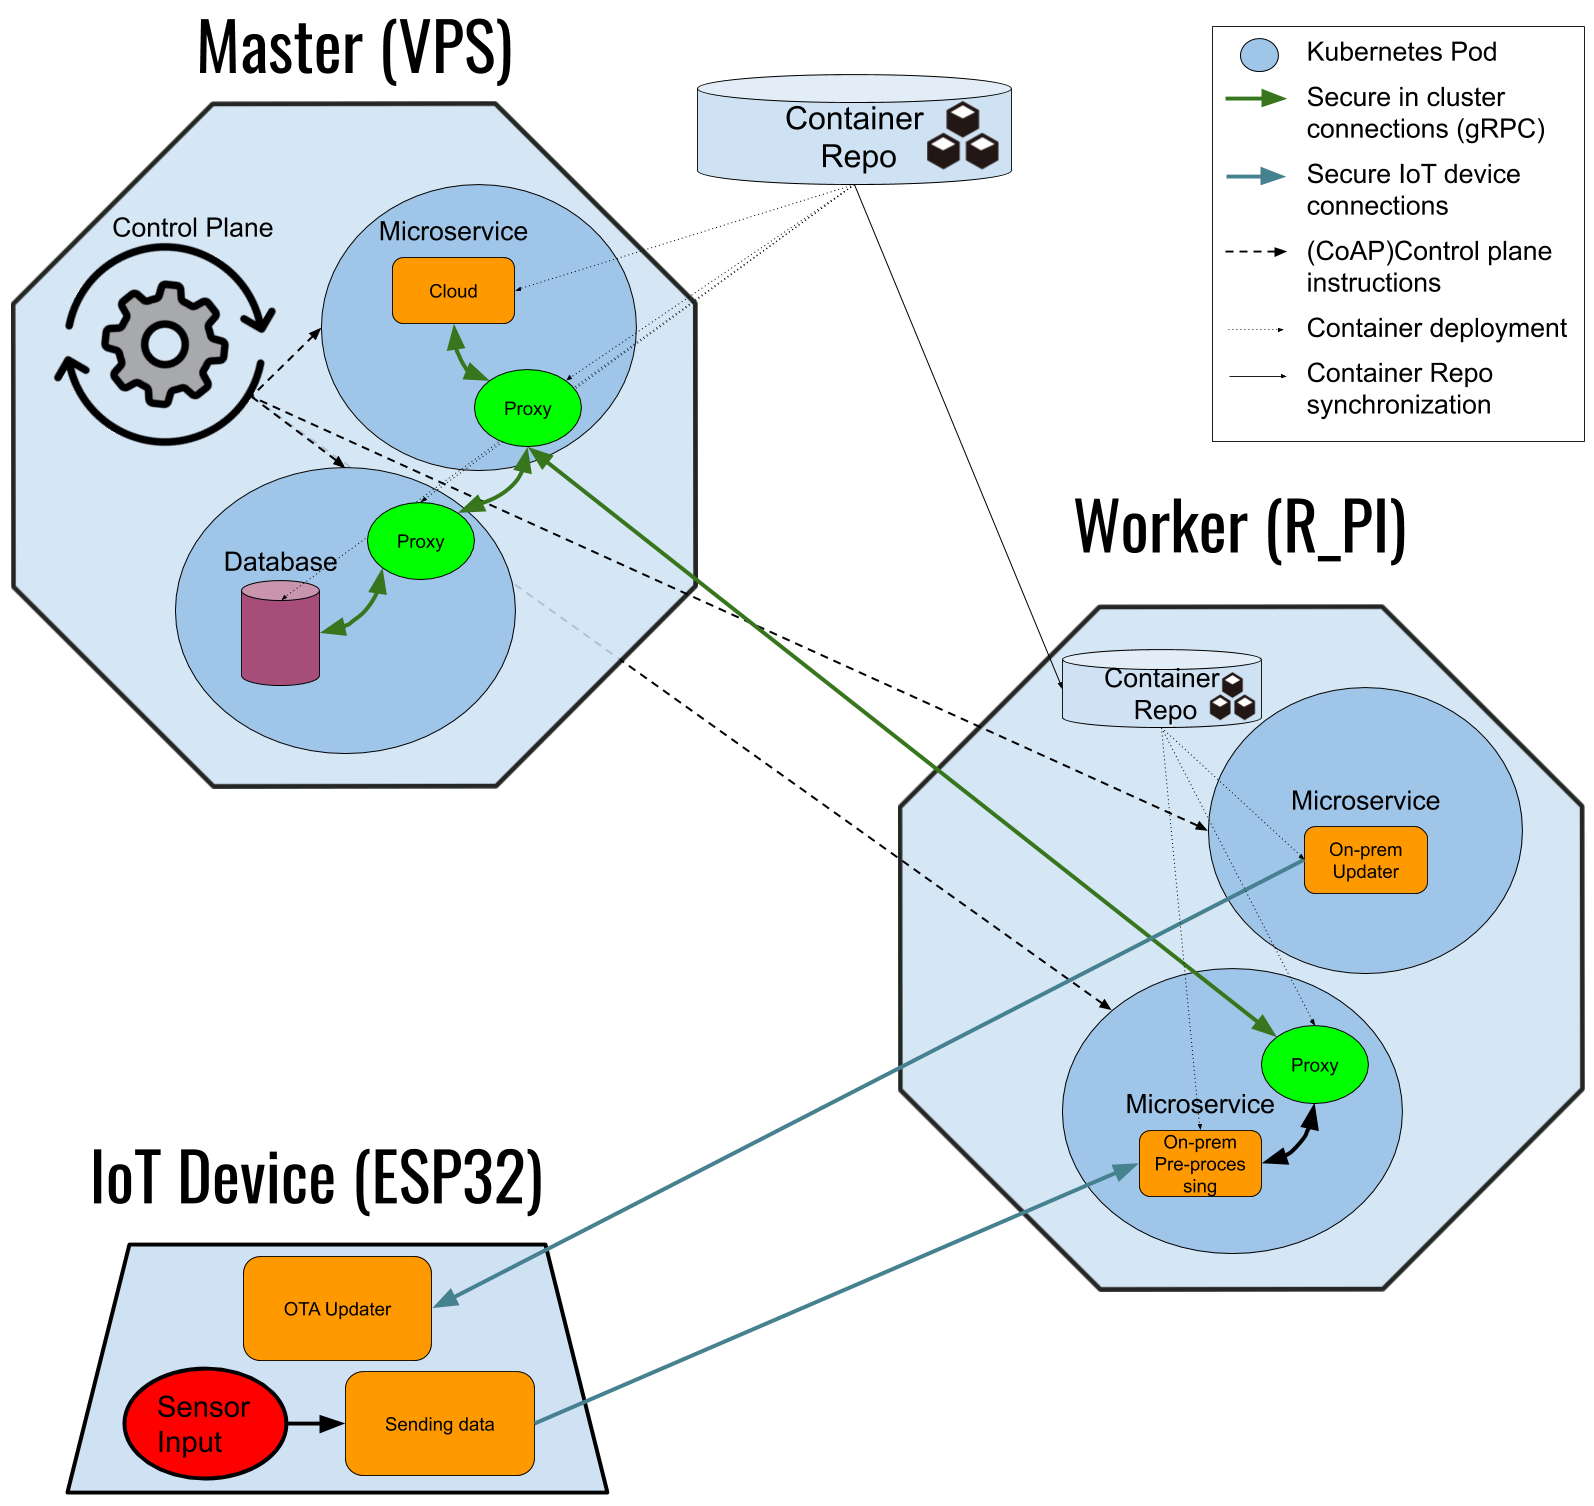
\includegraphics[scale=0.25]{figures/implementationSetup.png}
    \caption{The Desired System Architecture}
    \label{fig:implementationSetup}
\end{figure}
It has one master node running in the cloud on a VPS. This node is the primary contact point for the system administrator. The administrator defines the desired state of the cluster and gives the specifications to the master. The master runs a control plane which works towards achieving the desired state. Here, the master runs a microservice to process the data from the IoT gateway and stores it in a distributed database. However, the database is only present on nodes which also contain the microservice, it should never be scheduled on an edge device. Istio is deployed to keep the traffic secure between the database and the microservice. It achieves this by placing a proxy container in each pod to which all traffic is redirected. It tunnels all communication inside gRPC service calls and encrypts them with mutual TLS. That is, both parties are required to show that they have a certificate from a valid certificate authority, another Istio component. So all cluster internal traffic going in and out of a pod first passes through the proxy where it is encrypted or decrypted and forwarded to the correct container inside the pod. In the figure, the proxies are the small green bubbles and the encrypted communication is shown by the green arrows.

All images for the containers are pulled from an external container repository with the ability to be mirrored. The only one doing this at the time of writing is the Docker Hub. Production images use the image digest to ensure no image manipulation and consistency between deployments. The repository for the edge relevant containers is mirrored to the edge device, a RPi. The pulling of containers is represented by the small black dotted line while the synchronization is a small black continuous line.

The RPi is fully controlled by the master node in the cloud and only schedules the pods it is supposed to schedule. It contains to services, one is for interacting with the IoT device and another one for updating the IoT device. The containers are pulled from the local container registry and only if that fails will the node contact the remote registry. 

Finally, the IoT device, an esp32, has a service listening for input from a sensor and another service listening for updates from its gateway. It connects to the gateway via WiFi and sends data via the CoAP protocol encrypted with DTLS.

This setup reflects the resource available for this thesis. The master node is running on a VPS and not bare metal, because there was no access to a bare metal server. It is a single cluster setup as the size of the project did not justify the added overhead of a multi-cluster setup.






\comment{In fact, a new Kubernetes IoT Working Group is investigating how it can provide a consistent deployment model for IoT cloud and IoT Edge.
https://blog.bosch-si.com/bosch-iot-suite/why-the-iot-needs-kubernetes/

WHTA is important for edge? 
small containers
internet access (function without)
security
Speed (kubelet)
protocols


}